\chapter{Ground-Truth Evaluation Protocols}

\section{Ball Static Ground-Truth Dataset}

\subsection{Dataset Design}

A 36-point static dataset was designed to evaluate ball localisation accuracy across a representative volume of the arena. The grid covers X at 3000, 4000, 5000~mm (3 positions, spanning the central third of the arena depth), Y at 1000, 1600, 2300~mm (3 positions, spanning most of the arena width), and Z at 200, 700, 1200, 1800~mm (4 heights, from near-floor to above head height).

Total: $3 \times 3 \times 4 = 36$ trials, labelled B001--B036.

\begin{figure}[h]
    \centering
    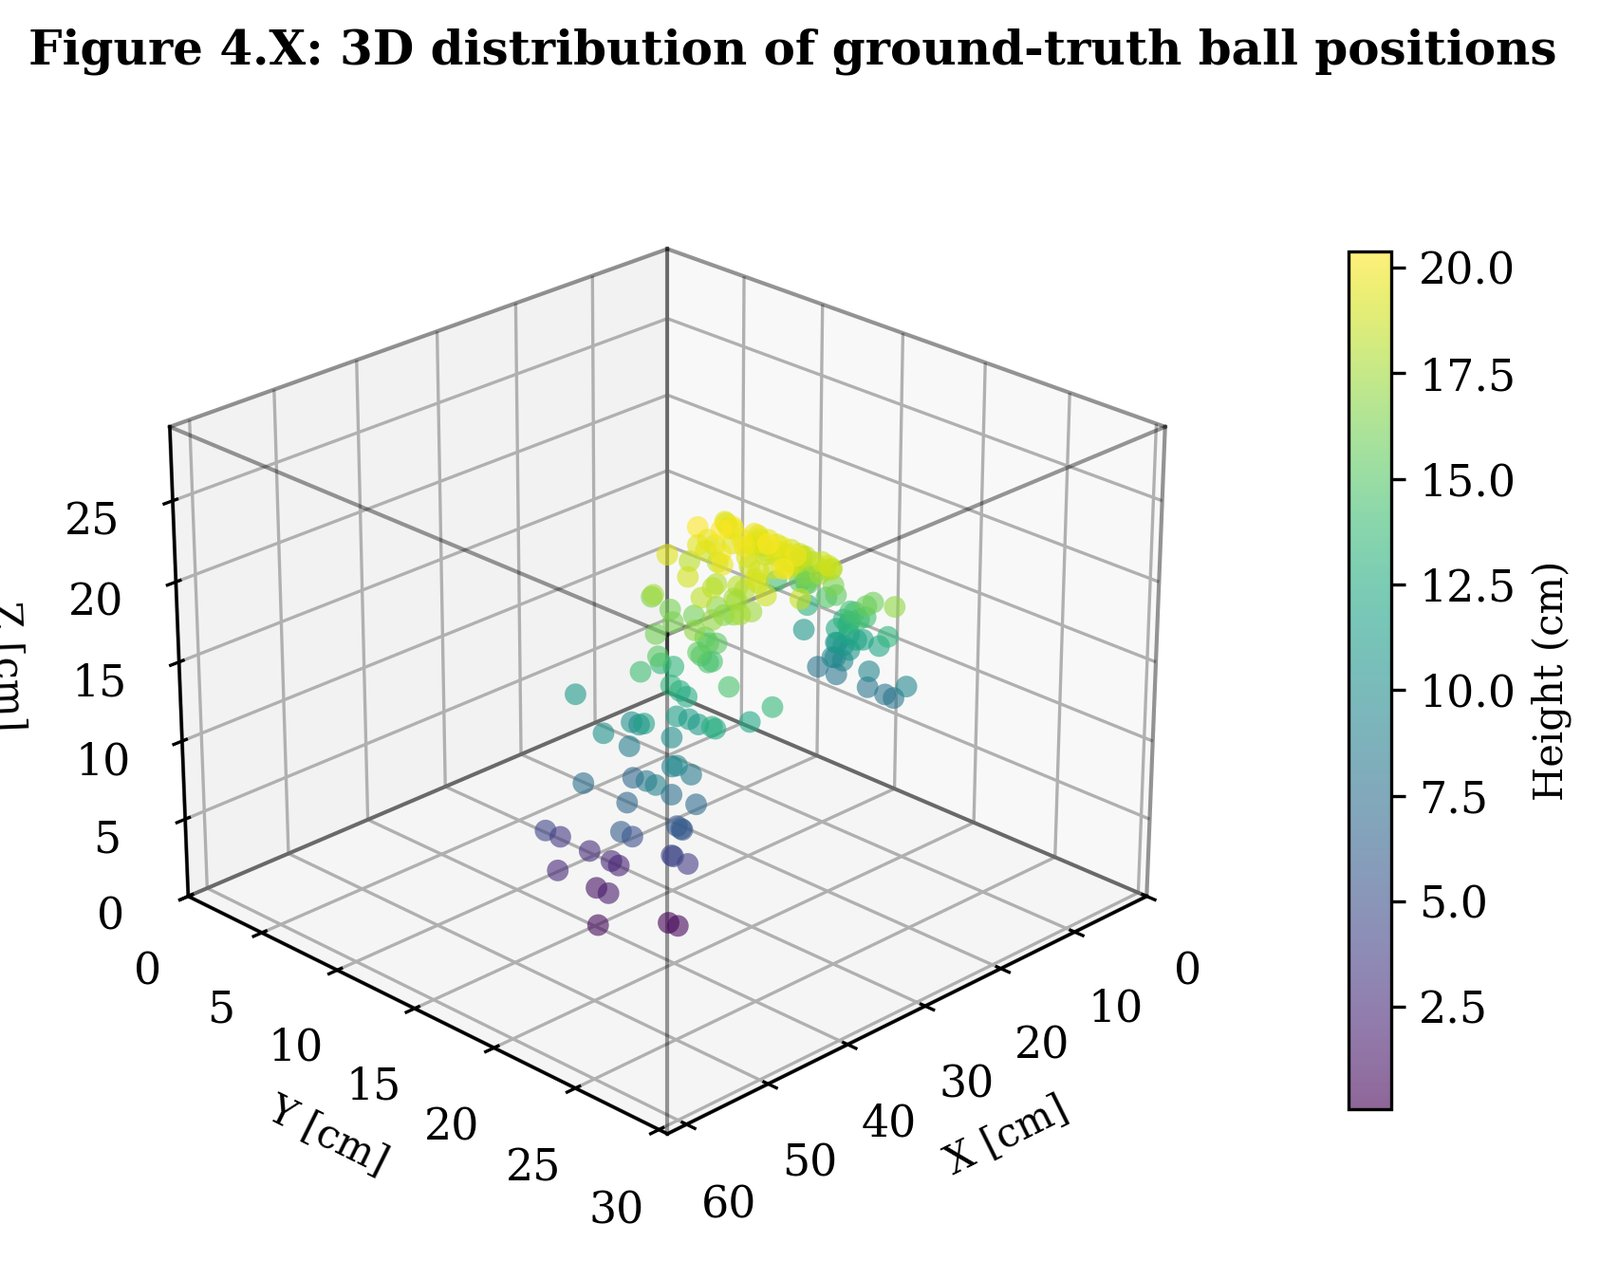
\includegraphics[width=0.8\textwidth]{figures/figure4_1_ball_static_gt_grid}
    \caption{Ball static GT grid: 36-point 3D scatter in arena frame.}
    \label{fig:4_1_ball_static_grid}
\end{figure}

\begin{table}[h]
    \centering
    \caption{Ball static ground-truth grid definition}
    \label{table:4_1_ball_static_grid}
    \begin{tabular}{|c|c|c|c|}
        \hline
        \textbf{X (mm)} & \textbf{Y (mm)} & \textbf{Z levels (mm)} & \textbf{Trial IDs} \\
        \hline
        3000 & 2300 & 200, 700, 1200, 1800 & B001, B010, B019, B028 \\
        \hline
        4000 & 2300 & 200, 700, 1200, 1800 & B002, B011, B020, B029 \\
        \hline
        5000 & 2300 & 200, 700, 1200, 1800 & B003, B012, B021, B030 \\
        \hline
        3000 & 1600 & 200, 700, 1200, 1800 & B004, B013, B022, B031 \\
        \hline
        4000 & 1600 & 200, 700, 1200, 1800 & B005, B014, B023, B032 \\
        \hline
        5000 & 1600 & 200, 700, 1200, 1800 & B006, B015, B024, B033 \\
        \hline
        3000 & 1000 & 200, 700, 1200, 1800 & B007, B016, B025, B034 \\
        \hline
        4000 & 1000 & 200, 700, 1200, 1800 & B008, B017, B026, B035 \\
        \hline
        5000 & 1000 & 200, 700, 1200, 1800 & B009, B018, B027, B036 \\
        \hline
    \end{tabular}
\end{table}

\subsection{Capture Protocol}

For each trial, a rigid holder positions the ball centre at the target coordinate, the scene is kept static for 3--4 seconds with all four cameras recording, and the trial ID and any anomalies are logged in \texttt{trials\_notes.csv}.

The ball centre position is measured physically using a tape measure referenced to the arena coordinate origin, with an estimated physical placement accuracy of $\pm 5$~mm.

\subsection{Processing}

Each trial's 4-camera clip is processed by \texttt{evaluate\_ball\_static\_gt.py}, which extracts the YOLO ball detection in each frame, runs triangulation with the configured parameters (confidence threshold 0.45, minimum 2 cameras, maximum reprojection error 14~px, EMA $\alpha = 0.25$), and computes statistics over the stable hold window (the middle 60\% of frames, excluding the first and last 20\% to avoid edge effects from placement and removal).


\section{Joint-Touch Ground-Truth Dataset}

\subsection{Dataset Design}

The joint-touch dataset evaluates the 3D localisation accuracy of three specific human joints under a controlled physical reference condition.

XY positions (9 points, $3 \times 3$ grid in central arena area):

\begin{table}[h]
    \centering
    \caption{Joint-touch trial design: XY grid positions (mm)}
    \label{table:4_2_joint_touch_xy}
    \begin{tabular}{|c|c|c|}
        \hline
        \textbf{XY Position Index} & \textbf{X (mm)} & \textbf{Y (mm)} \\
        \hline
        1 & 2600 & 1100 \\
        \hline
        2 & 3200 & 1100 \\
        \hline
        3 & 3800 & 1100 \\
        \hline
        4 & 2600 & 1600 \\
        \hline
        5 & 3200 & 1600 \\
        \hline
        6 & 3800 & 1600 \\
        \hline
        7 & 2600 & 2100 \\
        \hline
        8 & 3200 & 2100 \\
        \hline
        9 & 3800 & 2100 \\
        \hline
    \end{tabular}
\end{table}

Platform heights (Z base): 0~mm, 400~mm, 640~mm (three rigid platforms of different heights).

Joints evaluated: \texttt{right\_knee}, \texttt{right\_hip}, \texttt{left\_shoulder}.

Expected joint heights above platform base are \texttt{right\_knee} at base + 500~mm, \texttt{right\_hip} at base + 1000~mm, and \texttt{left\_shoulder} at base + 1560~mm.

Total trials: $9 \text{ positions} \times 3 \text{ heights} \times 3 \text{ joints} = 81$ trials, labelled J001--J081.

\begin{figure}[h]
    \centering
    
\includegraphics[width=0.8\textwidth]{figures/figure4_2_joint_touch_grid}
    \caption{Joint-touch trial grid: 9 XY positions and 3 height levels.}
    \label{fig:4_2_joint_touch_grid}
\end{figure}

\begin{table}[h]
    \centering
    \caption{Joint-touch platform and joint heights}
    \label{table:4_2b_joint_heights}
    \begin{tabular}{|c|c|c|c|c|}
        \hline
        \textbf{Platform Level} & \textbf{Z base (mm)} & \textbf{right\_knee Z} & \textbf{right\_hip Z} & \textbf{left\_shoulder Z} \\
        \hline
        Floor & 0 & 500 & 1000 & 1560 \\
        \hline
        Platform 1 & 400 & 900 & 1400 & 1960 \\
        \hline
        Platform 2 & 640 & 1140 & 1640 & 2200 \\
        \hline
    \end{tabular}
\end{table}

\subsection{Capture Protocol}

For each trial, the subject stands with the designated body joint touching a physical target marker placed at the specified XY position and height. The subject holds the position statically for 3--4 seconds. Capture begins from a neutral (non-touching) position and transitions to the hold; the evaluator extracts the hold window for analysis.

Validity criteria: a trial is valid if the joint is detected in at least 3 cameras during the hold window, the detection ratio (frames with valid detection / total frames in hold window) is $\geq 0.80$, and no obvious physical placement error was noted in the trial log.

Of 81 trials, 62 were classified as valid (76.5\% validity rate). The 19 invalid trials were mostly because of the camera visibility (the joint was occluded by the subject's own body from some camera angles) or the detection ratio was below threshold.

\subsection{Processing}

For each valid trial's 4-camera clip, MMPose inference with confidence threshold 0.35, minimum 3 cameras for pose triangulation, maximum reprojection error 14~px, and EMA $\alpha = 0.25$ is applied. The triangulated 3D position value within the hold window is computed as a mean value and is compared to the physical reference position.


\section{Dynamic Validation Clips}

Successive dynamic validation clips were recorded to evaluate the behaviour of the system in non-static conditions. The \texttt{ball\_slow} clip (20 seconds) involves the ball being gently moved with hand in the form of arcs and straight lines with the velocity of motion about 0.2--0.8~m/s; its purpose is to evaluate temporal tracking stability and continuous 3D trajectory reconstruction, with a pass criterion of no more than 3D frame-to-frame jumps of less than 800~mm. The \texttt{ball\_fast} clip (20 seconds) consists of real throws through the centre of the arena with normal playing speeds with changes in direction and close to wall trajectories; its purpose is to stress-test detection under motion blur and rapid acceleration, with a pass criterion of acceptable detection coverage, outlier rate controlled, and all detected points within arena bounds. The \texttt{no\_ball} clip (15 seconds) has the ball removed from the scene under normal arena lighting with a person present and moving; its purpose is to measure false-positive ball detection rate, with a pass criterion of false positive count close to zero.


\section{Error Metrics and Bias Correction Model}

\subsection{Primary Metrics}

For each trial, the 3D Euclidean error is computed as:

\begin{equation}
e = \sqrt{(x_{\text{est}} - x_{\text{gt}})^2 + (y_{\text{est}} - y_{\text{gt}})^2 + (z_{\text{est}} - z_{\text{gt}})^2}
\label{eqn:4_1_euclidean_error}
\end{equation}

where $(x_{\text{est}}, y_{\text{est}}, z_{\text{est}})$ is the mean estimated 3D position over the hold window and $(x_{\text{gt}}, y_{\text{gt}}, z_{\text{gt}})$ is the physical reference position.

Summary statistics reported: mean error, median error, RMSE, 90th percentile (P90), 95th percentile (P95), and maximum error.

\subsection{Axis Bias and Correction Model}

Systematic errors in camera calibration manifest as biases in the estimated 3D positions. Per-axis bias vectors are computed as:

\begin{equation}
\text{bias}_X = \text{mean}(x_{\text{est}} - x_{\text{gt}}) \text{ over all trials}
\label{eqn:4_2_bias_x}
\end{equation}

\begin{equation}
\text{bias}_Y = \text{mean}(y_{\text{est}} - y_{\text{gt}}) \text{ over all trials}
\label{eqn:4_3_bias_y}
\end{equation}

\begin{equation}
\text{bias}_Z = \text{mean}(z_{\text{est}} - z_{\text{gt}}) \text{ over all trials}
\label{eqn:4_4_bias_z}
\end{equation}

A linear correction model fits a scale and offset per axis to minimise residual error after correction. The corrected estimate is:

\begin{equation}
x_{\text{corr}} = (x_{\text{est}} - \text{bias}_X) \cdot \text{scale}_X
\label{eqn:4_5_x_correction}
\end{equation}

Analogous expressions apply for Y and Z. The pipeline results reported in Chapter~5 use the corrected model. It should be noted that the bias and scale parameters were estimated from the same 36-point static ball dataset used for final accuracy reporting; an independent held-out calibration set was not used. The correction therefore reflects in-sample fitting, and the reported corrected errors may underestimate the true generalisation error. This limitation should be considered when interpreting the corrected accuracy figures.

\section{Pose Backend Ablation Protocol}

To compare the YOLO-Pose backend against the MMPose reference back-end, an offline ablation study was conducted on three recorded motion sequences. The sequences (\textit{walk}, \textit{jog}, \textit{jump}) were captured under the same multi-camera arrangement as the joint-touch protocol but at a higher frame rate to provide 449 frames per camera, for a total of $449 \times 4 = 1796$ per-camera observations per sequence.

The protocol cached the 2D keypoint outputs of each pose backend for every frame, ran the standard multi-view DLT/SVD triangulation pipeline against both caches, and compared the resulting 3D joint trajectories. The principal outputs are: (i) the per-sequence detection rate (fraction of frames in which at least three cameras report a valid joint observation), (ii) the per-sequence inference latency (per-image and four-image batched), and (iii) the per-sequence 3D jitter (running standard deviation of the smoothed 3D joint position) compared between the two back-ends.

\section{Kalman-Prediction Tuning Protocol}

To select the constant-velocity Kalman-filter parameters used in the live runtime, a tuning grid was evaluated on the same three motion sequences. The grid swept process noise $q \in \{50, 200, 500, 1500\}$~mm$^{2}$/s$^{4}$ and measurement noise $r \in \{1, 10, 80, 250\}$~mm$^{2}$, with prediction horizons $\Delta t_{\text{pred}} \in \{0, 100, 200, 400, 600\}$~ms. For each grid point, the protocol computed the prediction error (the Euclidean distance between the Kalman-predicted joint position at time $t + \Delta t_{\text{pred}}$ and the actually-measured joint position at that future time) and reported the median, P90, and P95 statistics across the sequence.

The protocol's pass criterion is a positive percentage improvement of the predicted-position error over the na\"{i}ve ``predict equal to current'' baseline, computed as $1 - \mathrm{error}_{\text{KF}} / \mathrm{error}_{\text{naive}}$. A negative improvement indicates that the Kalman prediction is worse than not predicting at all; this is the expected outcome for highly non-linear motion under a constant-velocity assumption (for example, the jump sequence at large horizons).

\section{Ball Detection Analyser Protocol}

A separate offline tool, \texttt{ball\_detection\_analyzer.py}, evaluates the ball-detector configuration on recorded sequences without running the full live pipeline. The tool accepts either per-camera frame folders or four-camera tiled mosaic videos as input. For each input, it sweeps the detector confidence threshold (typically across $\{0.10, 0.15, 0.20, 0.25, 0.30, 0.40\}$) and the input image size (typically 672 and 960). For each (confidence, image-size) pair, it reports per-camera detection rate, multi-box (false-positive risk) frequency, the bounding-box aspect-ratio histogram (a proxy for motion blur), and the recovered detections relative to the production default (confidence~0.40, top-1).

A complementary offline mosaic renderer overlays the analyser's per-frame bounding boxes back on the four-camera tiled video, scaling per-camera-pixel coordinates to the tile dimensions and drawing a centre cross at each detection so that false-positive and false-negative modes can be inspected visually frame by frame.

\section{BLM Integration Protocol}

The integrated perception-to-actuation pipeline is validated through the six-stage BLM integration protocol (Appendix~A), which is summarised here for the reader's convenience.

\textbf{Stage S0 --- Serial connectivity.} The runtime opens \texttt{/dev/ttyUSB0} at 921~600~baud, sends \texttt{info}, and verifies a well-formed response within 500~ms.

\textbf{Stage S1 --- Manual command verification.} Each of \texttt{set}, \texttt{center}, \texttt{stop}, \texttt{shoot}, \texttt{reload}, \texttt{jv}, \texttt{jh} is sent via the raw serial terminal and the resulting physical motion is observed and matched against the \texttt{info} response. Pass criterion: every command produces the expected physical motion with no firmware reset.

\textbf{Stage S2 --- Runtime without cameras.} The runtime accepts synthetic UDP target packets and dispatches the resulting \texttt{set} commands; out-of-zone targets are logged as \texttt{OUT\_OF\_RANGE} and noisy targets as \texttt{LOW\_CONFIDENCE}. Pass criterion: every safety-gate categorical decision is correctly triggered.

\textbf{Stage S3 --- Live aim-only.} The full pipeline runs against live cameras with motors active and no ball loaded. Pass criterion: the launcher follows each of \texttt{right\_knee}, \texttt{right\_hip}, \texttt{left\_shoulder} with $<1^\circ$ steady-state error at stand-still and $<3^\circ$ during slow walk, and returns to centre between aims.

\textbf{Stage S4 --- Safety verification.} E-STOP response time, latch behaviour, and UDP/serial link-loss recovery are exercised under live conditions. Pass criterion: E-STOP triggers stop in $<$~100~ms; the system stays blocked until \texttt{clear} is issued; link loss triggers an automatic safe stop.

\textbf{Stage S5 --- Controlled fire.} Single shots are dispatched with a ball loaded, at low pitch (15$^\circ$) and moderate RPM (500), with the operator behind the launcher; the configuration is escalated stepwise to 600 and 800~RPM. Pass criterion: the ball trajectory reaches the intended zone with no mechanical anomaly, and exactly one shot is dispatched per trigger.

\textbf{Stage S6 --- Full-cycle reliability.} Ten consecutive aim$\to$shoot$\to$reload cycles are run. Pass criterion: no crash, no unsafe behaviour, and a complete JSONL log for each cycle.

Stages S0--S4, together with the integrated live test reported in Section~5.9, were completed on 2026-04-09. The integrated live test exercised the full reload$\to$aim$\to$shoot cycle on three named joints under operator supervision, in a configuration that exposed the closed-loop pipeline to a static and live-aim human target. Stage~S5/S6 in the moving-target regime is identified as future work in Section~6.4.
